\documentclass[a4paper,11pt,fleqn,oneside, openright]{memoir} % Brug openright hvis chapters skal starte p� h�jresider; openany, oneside

%%%% PACKAGES %%%%

% �� Overs�ttelse og tegns�tning �� %
\usepackage[utf8]{inputenc}					% G�r det muligt at bruge �, � og � i sine .tex-filer
\usepackage[danish]{babel}							% Dansk sporg, f.eks. tabel, figur og kapitel
\usepackage[T1]{fontenc}								% Hj�lper med orddeling ved �, � og �. S�tter fontene til at %v�re ps-fonte, i stedet for bmp	
\usepackage{latexsym}										% LaTeX symboler
\usepackage{xcolor,ragged2e,fix-cm}			% Justering af elementer
\usepackage{pdfpages}										% G�r det muligt at inkludere pdf-dokumenter med kommandoen \includepdf[pages={x-y}]{fil.pdf}	
\pretolerance=2500 											% G�r det muligt at justre afstanden med ord (h�jt tal, mindre orddeling og mere space mellem ord)
\usepackage{ulem}                       % Gennemstregning af ord med koden \sout{}
\usepackage{fixltx2e}										% Retter forskellige bugs i LaTeX-kernen
\usepackage{gensymb}					%Tilføjer \celsius og \degree notation	
\usepackage{lineno}						%Bruges til at tilføje linjetal
																	
% �� Figurer og tabeller � floats  �� %
\usepackage{flafter}										% S�rger for at dine floats ikke optr�der i teksten f�r de er sat ind.
\usepackage{multirow}                		% Fletning af r�kker
\usepackage{hhline}                   	% Dobbelte horisontale linier
\usepackage{multicol}         	        % Fletning af kolonner
\usepackage{colortbl} 									% Mulig�re farver i tabeller
%\usepackage{float}												% G�r det muligt at placere figurer hvor du vil.   \begin{figure}[!h] % Will not be floating.
\usepackage{wrapfig}										% Inds�ttelse af figurer omsv�bt af tekst. \begin{wrapfigure}{Placering}{St�rrelse}
\usepackage{graphicx} 									% Pakke til jpeg/png billeder
\pdfoptionpdfminorversion=6							% Muligg�r inkludering af pdf dokumenter, af version 1.6 og h�jere
	
% �� Matematiske formler og maskinkode ��
\usepackage{amsmath,amssymb,stmaryrd} 	% Bedre matematik og ekstra fonte
\usepackage{textcomp}                 	% Adgang til tekstsymboler
\usepackage{mathtools}									% Udvidelse af amsmath-pakken. 
\usepackage{eso-pic}										% Tilf�j billedekommandoer p� hver side
\usepackage{lipsum}											% Dummy text \lipsum[..]
\usepackage{rsphrase}										% Kemi-pakke til RS-s�tninger
\usepackage[version=3]{mhchem} 					% Kemi-pakke til lettere notation af formler

% �� Referencer, bibtex og url'er �� %
\usepackage{url}												% Til at s�tte urler op med. Virker sammen med hyperref
\usepackage[danish]{varioref}						% Giver flere bedre mulighed for at lave krydshenvisninger
\usepackage{natbib}											% Litteraturliste med forfatter-�r og nummerede referencer
\usepackage{xr}													% Referencer til eksternt dokument med \externaldocument{<NAVN>}

% �� Floats �� %
%\let\newfloat\relax 										% Memoir har allerede defineret denne, men det g�r float pakken ogs�
%\usepackage{float}

\usepackage[footnote,draft,danish,silent,nomargin]{fixme}		% Inds�t rettelser og lignende med \fixme{...} Med final i stedet for draft, udl�ses en error 																															for hver fixme, der ikke er slettet, n�r rapporten bygges.

%%%% CUSTOM SETTINGS %%%%

% �� Marginer �� %
\setlrmarginsandblock{3.5cm}{2.5cm}{*}	% \setlrmarginsandblock{Indbinding}{Kant}{Ratio}
\setulmarginsandblock{2.5cm}{3.0cm}{*}	% \setulmarginsandblock{Top}{Bund}{Ratio}
\checkandfixthelayout 									% Laver forskellige beregninger og s�tter de almindelige l�ngder op til brug ikke memoir pakker

%	�� Afsnitsformatering �� %
\setlength{\parindent}{0mm}           	% St�rrelse af indryk
\setlength{\parskip}{4mm}          			% Afstand mellem afsnit ved brug af double Enter
\linespread{1,1}												% Linie afstand

% �� Litteraturlisten �� %
\bibpunct[,]{[}{]}{;}{a}{,}{,} 					% Definerer de 6 parametre ved Harvard henvisning (bl.a. parantestype og seperatortegn)
%\bibliographystyle{bibtex/harvard}			% Udseende af litteraturlisten. Ligner dk-apali - mvh Klein

% �� Indholdsfortegnelse �� %
\setsecnumdepth{subsection}		 					% Dybden af nummerede overkrifter (part/chapter/section/subsection)
\maxsecnumdepth{subsection}							% �ndring af dokumentklassens gr�nse for nummereringsdybde
\settocdepth{section} 								% Dybden af indholdsfortegnelsen

% �� Visuelle referencer �� %
\usepackage[colorlinks=true]{hyperref}			 	% Giver mulighed for at ens referencer bliver til klikbare hyperlinks. .. [colorlinks]{..}
\hypersetup{pdfborder = 0}							% Fjerner ramme omkring links i fx indholsfotegnelsen og ved kildehenvisninger ��
\hypersetup{														%	Ops�tning af farvede hyperlinks
    colorlinks = true,
    linkcolor = black,
    anchorcolor = black,
    citecolor = black,
    urlcolor = black
}

\definecolor{gray}{gray}{0.80}					% Definerer farven gr�

% �� Ops�tning af figur- og tabeltekst �� %
 	\captionnamefont{
 		\small\bfseries\itshape}						% Ops�tning af tekstdelen ("Figur" eller "Tabel")
  \captiontitlefont{\small}							% Ops�tning af nummerering
  \captiondelim{. }											% Seperator mellem nummerering og figurtekst
  \hangcaption													%	Venstrejusterer flere-liniers figurtekst under hinanden
  \captionwidth{\linewidth}							% Bredden af figurteksten
	\setlength{\belowcaptionskip}{10pt}		% Afstand under figurteksten
		
% �� Navngivning �� %
\addto\captionsdanish{
	\renewcommand\appendixname{Appendiks}
	\renewcommand\contentsname{Indholdsfortegnelse}	
	\renewcommand\appendixpagename{Appendiks}
%	\renewcommand\cftchaptername{\chaptername~}				% Skriver "Kapitel" foran kapitlerne i indholdsfortegnelsen
	\renewcommand\cftappendixname{\appendixname~}			% Skriver "Appendiks" foran bilagene i indholdsfortegnelsen
	\renewcommand\appendixtocname{Appendiks}
}

% �� Kapiteludssende �� %
\definecolor{numbercolor}{gray}{0.7}			% Definerer en farve til brug til kapiteludseende
\newif\ifchapternonum

\makechapterstyle{jenor}{									% Definerer kapiteludseende -->
  \renewcommand\printchaptername{}
  \renewcommand\printchapternum{}
  \renewcommand\printchapternonum{\chapternonumtrue}
  \renewcommand\chaptitlefont{\fontfamily{pbk}\fontseries{db}\fontshape{n}\fontsize{25}{35}\selectfont\raggedleft}
  \renewcommand\chapnumfont{\fontfamily{pbk}\fontseries{m}\fontshape{n}\fontsize{1in}{0in}\selectfont\color{numbercolor}}
  \renewcommand\printchaptertitle[1]{%
    \noindent
    \ifchapternonum
    \begin{tabularx}{\textwidth}{X}
    {\let\\\newline\chaptitlefont ##1\par} 
    \end{tabularx}
    \par\vskip-2.5mm\hrule
    \else
    \begin{tabularx}{\textwidth}{Xl}
    {\parbox[b]{\linewidth}{\chaptitlefont ##1}} & \raisebox{-15pt}{\chapnumfont \thechapter}
    \end{tabularx}
    \par\vskip2mm\hrule
    \fi
  }
}																						% <--

\chapterstyle{jenor}												% Valg af kapiteludseende - dette kan udskiftes efter �nske

% �� Sidehoved �� %

%\makepagestyle{custom}																				% Definerer sidehoved og sidefod - kan modificeres efter �nske -->
%\makepsmarks{custom}{																						
%\def\chaptermark##1{\markboth{\itshape\thechapter. ##1}{}}		% Henter kapitlet den p�g�ldende side h�rer under med kommandoen \leftmark. \itshape g�r teksten kursiv
%\def\sectionmark##1{\markright{\thesection. ##1}{}}					% Henter afsnittet den p�g�ldende side h�rer under med kommandoen \rightmark
%}																														% Sidetallet skrives med kommandoen \thepage	
%\makeevenhead{custom}{Gruppe B130}{}{\leftmark}							% Definerer lige siders sidehoved efter modellen \makeevenhead{Navn}{Venstre}{Center}{H�jre}
%\makeoddhead{custom}{\rightmark}{}{Aalborg Universitet}			% Definerer ulige siders sidehoved efter modellen \makeoddhead{Navn}{Venstre}{Center}{H�jre}
%\makeevenfoot{custom}{\thepage}{}{}													% Definerer lige siders sidefod efter modellen \makeevenfoot{Navn}{Venstre}{Center}{H�jre}
%\makeoddfoot{custom}{}{}{\thepage}														% Definerer ulige siders sidefod efter modellen \makeoddfoot{Navn}{Venstre}{Center}{H�jre}		
%\makeheadrule{custom}{\textwidth}{0.5pt}											% Tilf�jer en streg under sidehovedets indhold
%\makefootrule{custom}{\textwidth}{0.5pt}{1mm}								% Tilf�jer en streg under sidefodens indhold

%\copypagestyle{nychapter}{custom}														% F�lgende linier s�rger for, at sidefoden bibeholdes p� kapitlets f�rste side
%\makeoddhead{nychapter}{}{}{}
%\makeevenhead{nychapter}{}{}{}
%\makeheadrule{nychapter}{\textwidth}{0pt}
%\aliaspagestyle{chapter}{nychapter}													% <--

\pagestyle{plain}																							% Valg af sidehoved og sidefod

% �� Fjerner den vertikale afstand mellem listeopstillinger og punktopstillinger �� %
\let\olditemize=\itemize							
\def\itemize{\olditemize\setlength{\itemsep}{-1ex}}
\let\oldenumerate=\enumerate						
\def\enumerate{\oldenumerate\setlength{\itemsep}{-1ex}}

%%%% CUSTOM COMMANDS %%%%

% �� Billede hack �� %
\newcommand{\figur}[4]{
		\begin{figure}[H] \centering
			\includegraphics[width=#1\textwidth]{billeder/#2}
			\caption{#3}\label{#4}
		\end{figure} 
}

% �� Specielle tegn �� %
\newcommand{\grader}{^{\circ}C}
\newcommand{\gr}{^{\circ}}
\newcommand{\g}{\cdot}

% �� Promille-hack (\promille) �� %
\newcommand{\promille}{%
  \relax\ifmmode\promillezeichen
        \else\leavevmode\(\mathsurround=0pt\promillezeichen\)\fi}
\newcommand{\promillezeichen}{%
  \kern-.05em%
  \raise.5ex\hbox{\the\scriptfont0 0}%
  \kern-.15em/\kern-.15em
  \lower.25ex\hbox{\the\scriptfont0 00}}

%%%% ORDDELING %%%%

\hyphenation{hvad hvem hvor}

%%%% Tabeler %%%%
\usepackage{threeparttable}
\usepackage[tableposition=top]{caption}

%%%% listings %%%%
\usepackage{listings}
\lstset{language=C}
\lstset{backgroundcolor=,rulecolor=}
\lstset{commentstyle=\textit}
\usepackage{lastpage}

\usepackage{marvosym}

%%%% top/tail %%%%

%\newcommand{\toptail}[1]{\fboxsep2mm\fbox{\begin{minipage}{145.3mm}#1\end{minipage}}}

\newcommand{\Ohm}{\ohm}
\newcommand{\my}{\mu}
\newcommand{\kilde}[1]{\fixme{Kilde: #1}}

 \usepackage[electronic]{ifsym}

\title{P3 Rapport}
\author{311}

\begin{document}
\thispagestyle{empty}
\begin{center}
\textsc{\huge Analog og digital elektronik\\}
\vspace{5 mm}

\textsc{\Large ...\\}
\vspace{25 mm}

\textsc{\textbf{\HUGE Effektforstærker\\}}
\vspace{20 mm}

\begin{flushright}
P3 Projekt \\
School of Information and Communication Technology \\
Elektronik \& IT Aalborg Universitet \\
Efteråret 2010 \\
\end{flushright}


\includegraphics[width=1.0\textwidth]{forside/forside.png}

\end{center}

%Blank side
\thispagestyle{empty}
\newpage
\mbox{}
\thispagestyle{empty}
\mbox{}
\newpage
\begin{multicols}{2}

\includegraphics[scale=0.35]{forside/aau.png}

\small{\textbf{Titel:\\}
HiFi-forstærker}

\scriptsize{\textbf{School of Information and Communication Technology\\ Elektronik \& IT\\}
Adresse: Fredrik Bajers Vej 7\\
Telefon: 99 40 86 00\\
URL: esn.aau.dk \\}
\end{multicols}
\begin{multicols}{2}

\small{
\textbf{Tema:\\}
Analog og digital elektronik

\textbf{Projektperiode:\\}
EIT3, efteråret 2010

\textbf{Projektgruppe:\\}
311

\textbf{Gruppemedlemmer:\\}
Benjamin Krebs\\
Frederik Juul\\
Jacob Hansen\\
Jesper Knudsen\\
Jonas Hansen\\

\textbf{Vejleder:\\}
Jan H. Mikkelsen

\textbf{Vikarierende vejleder:\\}
Ole Kiel Jensen

\textbf{Sidetal:\\}
\pageref{LastPage}

\textbf{Oplagstal:\\}
7

\textbf{Bilagsantal og art:\\}
1 bilags-CD

\textbf{Afsluttet den:\\}
21/12-2010
\\
\textbf{Synopsis:}
}

\fbox{\begin{minipage}{2.8in}
Der er i dette projekt arbejdet med design og fremstilling af en HiFi-forstærker. Målet med en HiFi-forstærker er at forstærke et lydsignal, med så stor præcision som muligt. Fra standarder er der opstillet en række krav som er valgt at overholde.

HiFi-forstærkeren i dette projekt består af fire moduler: Forforstærker, indgangsvælger, volumenkontrol og effektforstærker. Forforstærkerens funktion er at forstærke et mikrofonsignal til linieniveau, for at det kan sendes ind på niveau med et liniesignal. Dette gør at de to signaler kan behandles éns.
Indgangsvælgeren benyttes til at vælge imellem mikrofonsignalet eller stereosignalet: Intet signal, begge signaler eller de enkelte signaler hver for sig kan vælges. Indgangsvælgeren samler desuden signalerne, og skalérer det endelige signal, så outputtet derfra altid vil være på samme niveau.
Volumenkontrollen dæmper det samlede signals amplitude, til et af brugeren ønsket niveau, for at formindske den endelige volumen.
Effektforstærkeren forstærker signalet, hvilket sørger for at der kan afsættes den krævede effekt i højtaleren.
\end{minipage}}
\newline
\end{multicols}

\textit{\scriptsize{Rapportens indhold er frit tilgængeligt, men offentliggørelse (med kildeangivelse) må kun ske efter aftale med forfatterne.}}
\newpage
\begin{multicols}{2}

\includegraphics[scale=0.35]{forside/aau.png}

\small{\textbf{Title:\\}
HiFi-amplifier}

\scriptsize{\textbf{School of Information and Communication Technology\\ Electronics \& IT\\}
Adress: Fredrik Bajers Vej 7\\
Telephone: 99 40 86 00\\
URL: esn.aau.dk \\}
\end{multicols}
\begin{multicols}{2}

\small{\textbf{Theme:\\}
Analog and digital electronics

\textbf{Project Period:\\}
P3, fall 2010

\textbf{Project Group:\\}
311

\textbf{Group Members:\\}
Benjamin Krebs\\
Frederik Juul\\
Jacob Hansen\\
Jesper Knudsen\\
Jonas Hansen\\

\textbf{Supervisor:\\}
Jan H. Mikkelsen

\textbf{Number of pages:\\}
\pageref{LastPage}

\textbf{Printed Copies:\\}
8

\textbf{Appendix Media:\\}
1 appendix-CD

\textbf{Finished:\\}
21/12-2010
\\
\textbf{Synopsis:}}

\fbox{\begin{minipage}{2.8in}

...

...

...

...

...

...

...

...

...

...

...

...

...

...

...

...

...

...

...

...

...

...

...

...

...

...

...

...

...

...

...

\end{minipage}}
\newline
\end{multicols}
\textit{\scriptsize{The content of this paper is freely available, but publication (with references) is only allowed with permission from the author.}}

\newpage
%Blank side
\thispagestyle{empty}
\mbox{}
\newpage

%Læsevejledning
\section*{Læsevejledning}
I denne rapport benyttes forskellige former for notation. Disse er som følger:

\begin{itemize}
\item \textbf{Henvisninger til litteratur} er markeret med $"$[1]$"$ hvor nummeret svarer til et nummer i litteraturlisten. Disse henvisninger er, i den elektroniske version af rapporten, links, så de kan klikkes på. Henvisninger som er brugt til en enkelt information er markeret umiddelbart efter denne information og henvisninger brugt til et helt afsnit er markeret umiddelbart efter afsnittet.

\item \textbf{Henvisninger til figur eller afsnit} er markeret med $"$se figur/afsnit x.x.x$"$ hvor nummeret svarer til afsnitsnummeret i indholdsfortegnelsen eller figurnummeret under en figur. Disse henvisninger er, i den elektroniske version af rapporten, links.

\item \textbf{Binære tal} markeres med et undersænket b. F.eks. "10011$_b$" 

\item \textbf{Accepttestafsnit} sluttes alle med en tabel, der opsummerer de opstillede krav i forhold til deres status. Der vil ikke blive henvist til denne tabel, udover her. Et bestået krav er markeret med "\checkmark" mens et ikke bestået krav markeres med "$\mathcal{X}$".
\end{itemize}
%Ordliste
\section*{Ordliste}
\begin{itemize}
\item \textbf{AAU} - Aalborg Universitet
\item \textbf{EMC} - Electromagnetic compatibility
\item \textbf{THD} - Total Harmonic Distortion
\end{itemize}

\newpage
%Forord
\chapter*{Forord}
\label{forord}
Denne rapport dokumenterer et 3. semester projekt, udarbejdet i perioden fra 2. september 2010 til 21. december 2010. Projektet er udført af gruppe 311 på Elektronik og IT-ingeniør uddannelsen på Aalborg Universitet. Temaet for dette semester er $"$Analog og digital elektronik$"$ og gruppen valgte $"$High Fidelity (Hi-Fi) forstærker med digital styring$"$ som undertema. I løbet af semesteret modtager gruppen undervisning i form af PE- og SE-kurser, som bliver holdt af Institut for Elektroniske Systemer. Gruppen tilegner sig desuden viden gennem en fri studieaktivitet. Omtalte kurser er:

\begin{table}[h]
\centering
\begin{tabular}{c c}
\textbf{PE-kurser:} & \textbf{SE-kurser:} \\
Måleteknik & Quasistatiske elektriske og magnetiske felter \\
Analog elektronik & Beregningsteknik indenfor elektronikområdet 1 \\
Tilbagekoblingsteori 1 & Grundlæggende AC-kredsløbsteori \\
Basal digitalteknik & \\
\end{tabular}
\label{tab:kurser1}
\end{table}
\begin{table}[h]
\centering
\begin{tabular}{c}
\textbf{Fri studieaktivitet:} \\
PCB design og fabrikation \\
\end{tabular}
\label{tab:kurser2}
\end{table}
Gruppen har i løbet af projektet bestræbet sig på at opbygge mest muligt af løsningen analogt, fremfor digitalt. Der er i løbet af rapporten nævnt, når et element er udviklet specielt med dette for øje.\\\\
Gruppe 311 består af: \\\\\\\\\\
\begin{table}[h]
\centering
\begin{tabular}{c c c}
$\overline{~~~~~~Benjamin~Krebs~~~~~~}$ & $\overline{~~~~~~Frederik~Juul~~~~~~}$ & $\overline{~~~~~~Jacob~Hansen~~~~~~}$\\
\end{tabular}
\label{tab:gruppemedlemmer1}
\end{table} \\\\\\
\begin{table}[h]
\centering
\begin{tabular}{c c}
$\overline{~~~~~~Jesper~Knudsen~~~~~~}$ & $\overline{~~~~~~Jonas~Hansen~~~~~~}$\\
\end{tabular}
\label{tab:gruppemedlemmer2}
\end{table}

%Blank side
\thispagestyle{empty}
\mbox{}

\newpage
\tableofcontents*

%Linjetal
\setpagewiselinenumbers
\modulolinenumbers[5]
\linenumbers

%Indledning
\section{Indledning}
\begin{frame}{Indledning}

\end{frame}

\chapter{Indledende analyse}
\label{indledende_analyse}
\section{HiFi-forstærkerens generelle opbygning}

\begin{figure}[h]
\centering
\includegraphics[scale=.6]{indledende_analyse/generel_effektforstaerker/forstaerker_opbygning.png}
\caption{Opbygning af HiFi-forstærker}
\label{}
\end{figure}
\section{Systemopbygning}
For at kunne finde krav til dette projekts HiFi-forstærker er det nødvendigt at vælge hvilke blokke denne skal bestå af. I dette projekt er der ikke udelukkende valgt at designe en HiFi-forstærker i sin simpleste form, men også at tilføje funktionalitetsudvidende elementer. Systemets opbygning, med adskilte funktionelle blokke, er illustreret på figur \ref{fig:hififorstaerker_opbygning}. Dette afsnit vil argumentere og forklare den valgte opbygning. 


\begin{figure}[h]
\centering
\includegraphics[scale=0.6]{indledende_analyse/systemopbygning/forstaerker_opbygning.png}
\caption{Opbygning af dette projekts HiFi-forstærker}
\label{fig:hififorstaerker_opbygning}
\end{figure}


\subsection*{Input blokke}
Det er valgt at der skal kunne tilsluttes to typer lydkilder til HiFi-forstærkeren; en mikrofon og en kilde som afgiver et liniesignal. Kilder som afgiver et liniesignal er blandt andre computere, de fleste mobiltelefoner og medieafspillere, hvilket er grundlaget for netop at vælge denne type indgang. 
Grundlaget for at vælge en mikrofonindgang er udelukkende for at kunne anvende en indgangsvælger og for ikke at lave to ens linjeindgange. Desuden præsenterer en mikrofonindgang en ny blok: forforstærker.

HiFi-forstærkeren skal udstyres med et frontpanel hvorpå alle knapper til justeringsmulighederne skal placeres, således at de er tilgængelige for brugeren. Justeringsmulighederne, som skal være tilgængelige for brugeren er equalizerbånd, volumen og valg af indgang.

\subsection*{Analoge blokke}

Udgangsspændningen fra en mikrofon er langt lavere end linieniveau. Derfor benyttes en forforstærker til at forstærke mikrofonens lave signal op på niveau med liniesignalet, således at de er sammenlignelige i resten af systemet.

For at kunne vælge 

Forforstærker
Indgangsvælger
Volumenkontrol
Tonekontrol
Effektforstærker

\subsection*{Digital styring}
Digital styring


\subsection*{Output blokke}
Displays
Monoudgang
\section{Standarder}
\label{standarder}
I dette afsnit bliver der taget udgangspunkt i gældende standarder fra International Electrotechnical Commitee (IEC) og Deutsches Institut f\"{u}r Normung (DIN). Målet med standarder er at opstille nogle normer for hvad produkter skal leve op til, hvilket gøres for at standardisere markedet sådan at produkter fra forskellige producenter kan arbejde sammen og ikke kun virker med produkter fra samme producent. Kravene opstillet i standarderne er ikke lovkrav, men derimod retningslinier. Det er dog i de færrestes interesse ikke at overholde standarderne.
\newline
\newline
I dette projekt er der valgt at arbejde med tre forskellige standarder. De tre standarder der arbejdes med er IEC581 Part 6, IEC61938 1 udgave og DIN 45500 normen.


\subsection*{IEC581 Part 6 - Amplifiers}
\label{IEC581}
Standarden IEC581 har titlen $"$High fidelity audio equipment and systems; Minimum performance requirements$"$ og er fra 1979. I dette projekt er det valgt kun at anvende del 6 af standarden da kun denne del har relevans for projektet. Del 6 af standarden opstiller generele minimumskrav til hvad en HiFi-forstærker skal overholde. \cite{IEC581-6}%\fixme{Kilde til IEC581-6}
\newline
\newline
Den første værdi der er taget fra standarden siger hvad minimumskrav der er for udgangseffekten.
\newline
\newline
\textbf{Udgangseffekt}
\begin{itemize}
\item Der skal minimum være et output på 10 W per kanal og det skal overholde kravet om forvrængning
\item Hvis forstærkeren har mere end én kanal skal alle kanaler kunne levere minimum 10 W samtidig.
\item Forstærkeren skal kunne levere det fastsatte output indenfor THD afvigelse i mindst 10 min., med alle kanaler tændt og en temperatur mellem 15 °C og 35 °C. Relativt til 1 kHz.
\end{itemize}

Den anden værdi der er taget fra standarden fastsætter et minimum for hvilket frekvensområde forstærkeren skal arbejde indenfor.
\newline 
\newline
\textbf{Frekvensområde}
\begin{itemize}
\item Frekvensområdet skal som minimum gå fra 40 Hz til 16 kHz
\item Der må være en tolerance på $\pm$ 1,5 dB for signaler der ikke er kommet igennem en equalizer. Relativt til 1 kHz
\item Der må være en tolerance på $\pm$ 2 dB for signaler der er kommet igennem en equalizer. Relativt til 1 kHz
\end{itemize}


\subsection*{IEC61938 1. udgave}
\label{IEC61938}
Standarden IEC61938 har titlen $"$Audio-, video- og audiovisuelle systemer - Indbyrdes forbindelser og matchende værdier - Foretrukne matchende analoge signalværdier$"$ og er fra 1997. Standarden der er brugt i rapporten er 1. udgave. Standarden opstiller generelle minimumskrav for hvad en HiFi-forstærker skal overholde. \cite{IEC61938}%\fixme{Kilde til IEC61938} 
\newline
\newline
Den første værdi fra standarden fremsætter hvad der skal overholdes for en linieindgang\fixme{Jesper: Skal nok lige skrives at der vælges en linie- og en mikrofonindgang før der kommer standarder for sjovt nok lige præcis de to typer}
\newline
\newline
\textbf{Liniesignaler}
\begin{itemize}
\item Indgangsimpedansen skal være større eller lig med 22 k\ohm
\item Signalspændingssvinget skal være mellem 0,2 V og 2 V
\item Udgangsimpedansen skal højst være 2,2 k\ohm
\end{itemize}
Anden krav fra standarden fremsætter hvad der skal overholdes for en mikrofonindgang
\newline 
\newline
\textbf{Mikrofonsignal}
\begin{itemize}
\item Indgangsimpedansen skal være større eller lig med 22 k\ohm
\item Outputspændingen skal være mellem 0,2 V og 2 V
\item Udgangsimpedansen skal højest være 2,2 k\ohm
\end{itemize}

\subsection*{DIN 45500 normen}
\label{DIN45500}
DIN 45500 normens fulde titel er Deutsches Institut f\"{u}r Normung 45500. Denne norm gælder for audioudstyr og er taget med fordi den opsætter minimumkrav til hvad en HiFi-forstærker skal overholde. Normen er fra 1973. \cite{DIN45500}%\fixme{Kilde til DIN45500}
\newline
\newline
Den første værdi fra normen beskriver hvor meget en HiFi-forstærker må forvrænge.
\newline
\newline
\textbf{Harmonisk forvrængning}
\begin{itemize}
\item Forforstærker eller effektforstærker må maksimalt forvrænge 0,7 \%
\item Forforstærker og effektforstærker må maksimalt forvrænge 1,0 \%
\item Dette skal være overholdt i en effektbåndbredde fra 40 Hz til 12,5 kHz
\end{itemize}
Den anden værdi fra normen beskriver krav til belastningsimpedansen.
\newline 
\newline
\textbf{Belastningsimpedans}
\begin{itemize}
\item For højtalere skal belastningsimpedansen være enten 4 \ohm~eller 8 \ohm
\item For hovedtelefoner skal belastningsimpendansen være enten 200 \ohm~eller 400 \ohm
\item Tolerance på 20 \%
\end{itemize}
\section{Equalizer}
\label{equalizer}
Det menneskellige øre kan opfatte frekvenser fra ca. 20-20k Hz\fixme{kilde: http://www.hoerelse.info/page.dsp?page=414}. Dette sætter en naturligt bredde for frekvensbåndet, forstærkeren skal kunne operere indenfor. Udover at en given elektrisk komponent ikke vil være ens over hele frekvensbåndet, vil det akustiske miljø samt højtalerne også have indflydelse på den endelige oplevelse.  Derfor kan det være nødvendigt at regulere på de forskellige frekvenser, for at opnå den ønskede lyd. En equalizer benyttes til at dæmpe de forskellige frekvensbånd, i forhold til hinanden. En equalizer i en forstærker vil ofte være bredspektret og blive benyttet til at korrigere mere generelle ændringer i lyden. Hvis brugeren ønsker mere specifikke indstillinger, vil en dedikeret equalizer ofte benyttes. Da frekvensbåndet det menneskelige øre kan høre består af præcis 3 dekader, inddeles frekvensbåndene i equalizeren efter disse:
%Udtrykket equalizer stammer fra den originale hensigt med opfindelsen; at få det optagede til at lyde som den originale kilde. Dette gøres bl.a. for at kompensere for unøjagtigheder i optagelsesudstyr. Ved at dæmpe og forstærke individuelle frekvensbånd, er det muligt at få præcis den lyd brugeren kunne tænke sig. 
%En equalizer i en forstærker vil ofte være bredspektret og blive benyttet til at kompensere for det akustiske miljø brugeren befinder sig i, samt unøjagtigheder som følge af de benyttede komponenter. Hvis man har brug for mere specifikke indstillinger vil benyttet en dedikeret equalizer. Derfor har projektgruppen valgt at have 3 frekvensbånd\fixme{kilde: pdf dokument.}.

\begin{itemize}
\item Low: 20 - 200 Hz
\item Mid: 200 - 2000 Hz
\item High: 2000 - 20000 Hz
\end{itemize}

%Frekvensbåndene strækker sig fra 20 Hz til 20 kHz, da dette er det maksimale frekvensbånd det menneskelige øre kan opfatte\fixme{kilde: http://www.hoerelse.info/page.dsp?page=414}. Da dette frekvensbånd består af præcis 3 dekader, har projektgruppen valgt at inddele equalizerens frekvensbånd i disse.
%Hvor mange indstillingmuligheder der er på en equalizer, afhænger af antal af frekvensbånd, som kan indstilles uafhængigt af hinanden. Der opstilles derfor en række frekvensbånd, som et mål for projektet:
%Idéen med en equalizer er at kunne justere på styrken af de forskellige frekvenser i et signal, uafhængigt af hinanden. Dette benyttes til at få præcis den lyd, som brugeren ønsker. Eksempelvis kunne en bruger vælge at skrue op for de lave frekvenser, for at gøre bassen i et signal mere dominerende. I praksis er det dog en kombination af at forstærke nogle frekvensbånd, og dæmpe andre, på tværs af hele det hørbare område, for at skabe nøjagtigt den lyd der ønskes.\fixme{Skriv om} Dette er en hel videnskab i sig selv, men for at gøre mulighederne for dette så store som muligt, er det smart\fixme{andet ord?} at have et bredt udvalg af justerbare bånd. Dette gøres, analogt, ved hjælp af forskellige båndpas filtre.

\subsection{Visualizer}
\label{visualizer}
Visualizeren benyttes til at illustrere styrken af de signalerne i de forskellige frekvensbånd. I teorien kan en analog visualizer have uendeligt stor opløsning. I dette projekt vil det dog ikke give mening, ud fra et læringsmæssigt standpunkt at lave for stor opløsning, da dette bare er gentagelse af de samme basale elementer. Derimod vil en for lav opløsning heller ikke kunne bruges til noget. Derfor er en opløsning på seks dioder pr. frekvensbånd valgt. Dette giver desuden mulighed for at vise signalstyrken med farver: 2 grønne, efterfulgt af 2 gule, efterfulgt af 2 røde dioder.
%En visualizer giver et visuelt udtryk for, hvordan equalizeren er indstillet. Den angiver lydniveauet for hvert frekvensbånd, equalizeren dækker over. Dette giver bl.a. brugeren mulighed for at se hvilke frekvenser, der vil være optimale at justere på, for at få det ønskede output.
\section{Total Harmonic Distortion}
\label{thd}
Total Harmonic Distortion, total harmonisk forvrængning - forkortet THD - er et udtryk for hvor meget forvrængning der er i et signal, fra kilden til output.  Hele kæden er med til at øge THD, da det er et biprodukt af, at komponenter ikke er lineære og derfor vil tilføje forvrængning til signalet. Jo højere THD, jo kraftigere overtoner, kendt på engelsk som harmonics\fixme{evt. i fodnote eller ordforklaring i stedet?}, vil der blive produceret, hvilket vil ændre det originale signal. Overtoner er frekvenser, som har et heltalsforhold\fixme{er det et ord?} til den originale frekvens; eksempelvis vil overtoner til 500Hz være 1000Hz, den dobbelte frekvens, og 1500Hz, tre gange frekvensen.\fixme{Skriv om med ligning} Disse overtoner bliver lagt til det originale signal; dette svarer til at det originale signal, er en slags AC-offset til de mindre kraftige overtoner, som set i figur \fixme{figur}. Det er derfor vigtigt at få så lav forvrængning som muligt, da hvert enkelt led i kæden, bidrager med sin egen. Så længe HiFi-forstærkerens totale forvrængning er under 1\% anses den dog som værende underordnet, da det ikke er muligt at detektere med det menneskelige øre.\fixme{kilde eller lav en ref til standarder}

\begin{figure}[h]
\centering
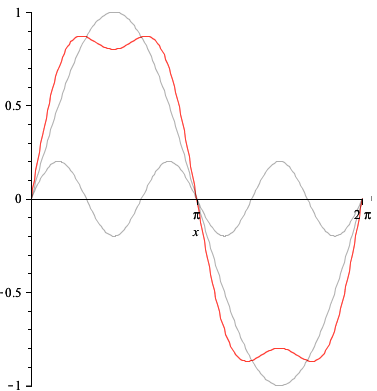
\includegraphics[scale=.4]{indledende_analyse/thd/thdsamlet.png}
\caption{Et eksempel på harmonisk forvrængning. Det originale signal virker som et AC-offset for den mindre kraftige, tredje harmoniske overtone.}
\label{fig:harmonic_distortion}
\end{figure}
\section{Klasser}
\label{klasser}
En HiFi-forstærkers udgangstrin kan designes på forskellige måder alt efter hvilken funktionalitet der ønskes. De forskellige designs er opdelt i klasser. Klasserne er bestemt ud fra en karakteristik og ikke ud fra en bestemt opkobling af kredsløbet. Karakteristika, som er vigtige at tage i betragtning for udgangstrinnet i en HiFi-forstærker er virkningsgrad, strømvinkel og forvrængning. Virkningsgrad er givet ved hvor stor en procentdel af den totale effekt leveret af forsyning, der bliver afsat i loaden, i dette tilfælde højtaleren.
I dette afsnit vil der blive gjort rede for klasse A, B og AB samt forklaret hvilke fordele og ulemper der er med dem. Redegørelsen vil tage udgangspunkt i ovenstående karakteristika samt demonstrere en mulig opbygning af trinnet.
Der vil, på baggrund af dette afsnit, blive valgt en endelig udgangstrinsklasse til dette projekts HiFi-forstærker hvilket vil blive, et krav i kravspecifikationen.

\subsection{Klasse A}

Et klasse A udgangstrin har en strømkarakteristik på udgangen, som vist på figur \ref{fig:klassea} med en sinustone, som indgangssignal. 

\begin{figure}[ht]
\begin{minipage}[b]{0.5\linewidth}
\centering
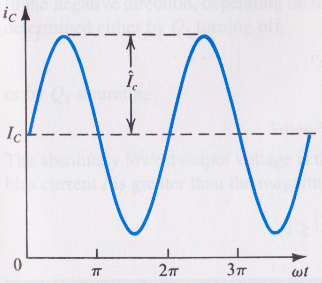
\includegraphics[scale=.35]{valg_af_loesning/klasser/klassea.png}
\caption{Klasse A $i_c$ karakteristik}
\label{fig:klassea}
\end{minipage}
\hspace{0.5cm}
\begin{minipage}[b]{0.5\linewidth}
\centering
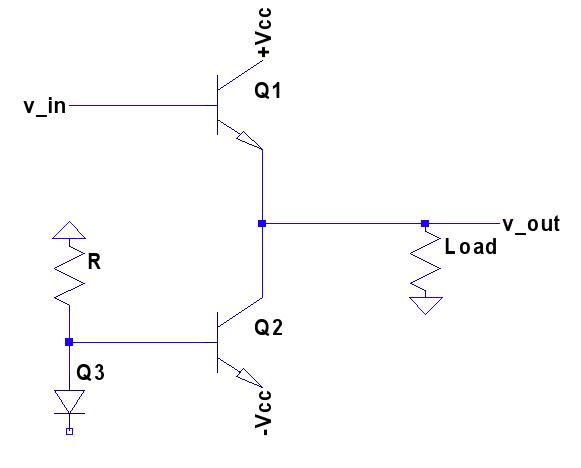
\includegraphics[scale=.35]{valg_af_loesning/klasser/classa.png}
\caption{Et eksempel på et klasse A forstærker kredsløb}
\label{fig:classa}
\end{minipage}
\end{figure}
\fixme{kilde: til sedra smith}


Et klasse A trin har en strømvinkel på udgangstransistoren på 360°. Dette viser sig nyttigt i det at indgangssignalet er repræsenteret på udgangen i sin komplette form, hvilket giver en lav forvrængning.
I et klasse A trin løber altid en konstant strøm gennem Q2, hvis kredsløbet på figur \ref{fig:classa} benyttes. Dette gør at den maksimale teoretiske virkningsgrad kun er 25\%. \fixme{kilde: til sedra smith}

Et klasse A udgangstrin kan opbygges af to NPN transistorer, Q1 og Q2, i en emitterfølgerkobling, som vist på figur \ref{fig:classa}. En konstant strøm løber gennem Q2, da $v_{BE2}$ er konstant. Inputsignalet kommer ind på Q1's base og styrer således strømmen der kan løbe gennem Q1 og loadmodstanden. 



\subsection{Klasse B}

Et klasse B udgangstrin har en strømkarakteristik på udgangen, som vist på figur \ref{fig:klasseb} med en sinustone, som indgangssignal. 

\begin{figure}[ht]
\begin{minipage}[b]{0.5\linewidth}
\centering
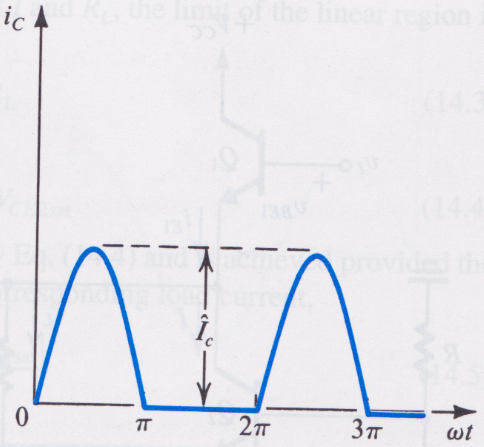
\includegraphics[scale=.35]{valg_af_loesning/klasser/klasseb.png}
\caption{Klasse B $i_c$ karakteristik}
\label{fig:klasseb}
\end{minipage}
\hspace{0.5cm}
\begin{minipage}[b]{0.5\linewidth}
\centering
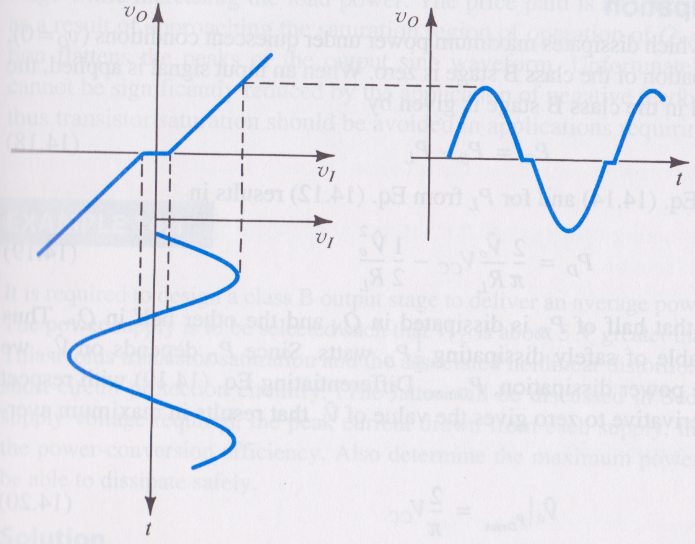
\includegraphics[scale=.25]{valg_af_loesning/klasser/klassebproblem.png}
\caption{Klasse B trin med crossoverdistortion}
\label{fig:classbproblem}
\end{minipage}
\end{figure}
\fixme{kilde: til sedra smith}
Et klasse B trin overfører kun en halv periode af indgangssignalet til udgangen, altså er strømvinklen 180°. For at kunne gengive et udgangssignal similært til indgangssignalet er det derfor nødvendigt at sammensætte to klasse B trin således at det ene tager sig af den positive halvperiode og den anden den negative. Dette giver anledning til et fænomen kaldet crossoverdistortion. Dette fænomen optræder i dette tilfælde i overgangen fra den positive halvperiode til den negative og skyldes diodekarakteristikken i transistorernes base-emitter. Crossoverdistortion for et klasse B trin er illustreret på figur \ref{fig:classbproblem}.
Et klasse B trin har en maksimal nyttevirkning på 78,5 \%.\fixme{kilde: til sedra smith}

I eksemplet er klasse B trinnet opbygget af to transistorer, en NPN (Q1) og en PNP (Q2), som vist på figur \ref{fig:classb}. Når input spændingen overstiger ca. 0,6 V vil Q1 begynde at lede strøm til loadmodstanden mens Q2 er lukket. Kommer input spændingen under -0,6 V vil Q2 lede, men da Q2 er en PNP vil den trække strøm mod -Vcc hvormed der trækkes strøm fra loadmodstanden. Når Q2 leder er Q1 lukket. 

\begin{figure}[h]
\centering
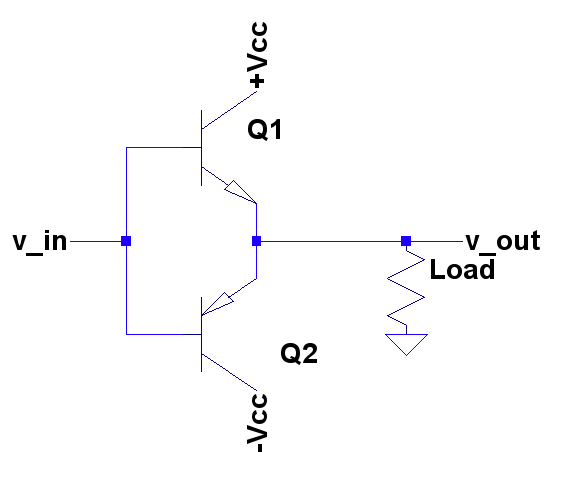
\includegraphics[scale=.35]{valg_af_loesning/klasser/classb.png}
\caption{Klasse B forstærker kredsløb}
\label{fig:classb}
\end{figure}

\subsection{Klasse AB}

Et klasse AB udgangstrin har en strømkarakteristik på udgangen, som vist på figur \ref{fig:klasseab} med en sinustone, som indgangssignal. 

\begin{figure}[ht]
\begin{minipage}[b]{0.5\linewidth}
\centering
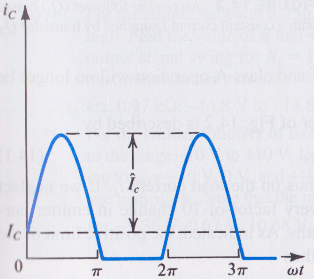
\includegraphics[scale=.35]{valg_af_loesning/klasser/klasseab.png}
\caption{Klasse AB $i_c$ karakteristik}
\label{fig:klasseab}
\end{minipage}
\hspace{0.5cm}
\begin{minipage}[b]{0.5\linewidth}
\centering
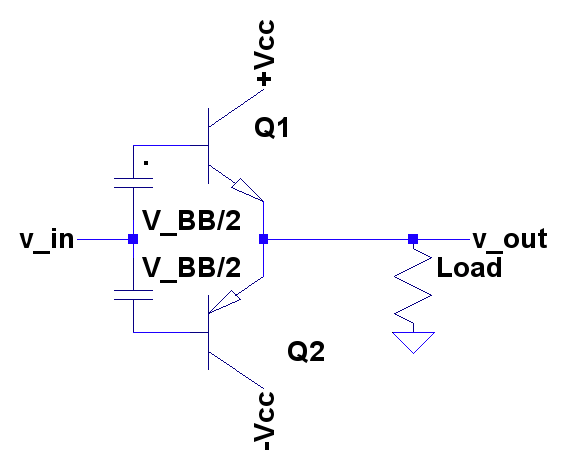
\includegraphics[scale=.35]{valg_af_loesning/klasser/classab.png}
\caption{Klasse AB forstærker kredsløb}
\label{fig:classab}
\end{minipage}
\end{figure}
\fixme{kilde: til sedra smith}


Dette trin har en strømvinkel på mellem 180 ° og 360 °. Dette bevirker at, hvis man bruger samme teknik, som ved et klasse B trin til at få en hel sinusperiode på udgangen, vil de to signaler overlappe i overgangsperioden. Dette medvirker til at crossoverdistortion, som forklaret for klasse B trinnet, elemineres. Dermed bliver forvrængningen for et klasse AB mindre end for et klasse B.
Et klasse AB trin har en nyttevirkning som ligger mellem den for et klasse A og et klasse B. \fixme{kilde: Jan ???}

Der tages i eksemplet på et klasse AB trin på figur \ref{fig:classab} udgangspunkt i klasse B trinnet på figur \ref{fig:classb}, med den forskel at potentialet på Q1 og Q2's base er hævet til saturationspændingen når signalspændningen er 0 V. Det er denne forskel, som eleminerer crossoverdistortion.

Et klasse AB udgangstrin har ikke et klasse A's lave nyttevirkning eller et klasse B's crossoverdistortion og er på baggrund af dette blevet valgt, som det udgangstrin der vil blive arbejdet videre på.

%Kravspecifikation
\chapter{Kravspecifikation}
\label{kravspec}
Formålet med dette kapitel er til slut at opstille en kravspecifikation for projektets HiFi-forstærker. Alle kravene i kravspecifikationen skal være målbare, så de kan testes ved projektets afslutning, og begrundede i det omfang dette er muligt. Før det er muligt at opstille en sådan kravspecifikation, er det nødvendigt at dokumentere hvilke overvejelser som danner grundlag for de forskellige dele af kravspecifikationen. Der er i kapitel \ref{kap:indledende_analyse} ført dokumentation for en række af disse overvejelser. De resterende overvejelser er dokumenteret i de næste syv afsnit. I afsnit \ref{krav_krav} er produktet af alle disse overvejelser samlet i den endelige kravspecifikation for projektets HiFi-forstærker. 

\section{Indgangsvælger}
\label{krav_indgangsvaelger}
I forbindelse med indgangsvælgeren er overvejelserne gået på, hvorvidt denne skal lave en trinvis eller flydende overgang mellem indgangssignalerne. Da en flydende overgang i princippet er simultan volumenkontrol af indgangene, adskiller den form for indgangsvælger sig ikke i samme grad fra en egentlig volumenkontrol, som det er tilfældet med en trinvis indgangsvælger. Eftersom der er opstillet krav om en volumenkontrol til forstærkeren sættes kravet om indgangsvælgerens art til trinvis. \\
Som det fremgår i afsnit \ref{standarder} skal HiFi-forstærkeren have to indgange, hvilket danner grundlag for at kravet til antallet af trin i indgangsvælgeren sættes til tre. De tre trin er vist i tabel \ref{tab:indgangsvaelgertrin}.\fixme{Jesper: Har ikke lavet det med isolation, da jeg vil vente og se hvad Jacob skriver om det - ¿ Mener jeg hørte han fandt noget med det til standarder ?}

\begin{table}[h]
\centering
\begin{tabular}{c|c|c}
\hline\hline
Trin & Indgang 1 & Indgang 2 \\
\hline\hline
1 & On & Off \\
2 & Off & On \\
3 & On & On \\
\hline\hline
\end{tabular}
\caption{Indgangsvælgertrin}
\label{tab:indgangsvaelgertrin}
\end{table}

Valget mellem de tre trin skal kunne tages af brugeren på HiFi-forstærkerens frontpanel. Det skal desuden være tydeligt hvilket trin indgangsvælgeren er sat på.

\section{Indgangsimpedans}
\label{krav_indgangsimpedans}
Indgangsimpedansen er at opfatte som en impedans der, ud fra en almindelig spændingsdeling, reducerer indgangssignalet. Man er, med den begrundelse, interesseret i en stor indgangsimpedans. Den mindste tilladte størrelse af indgangsimpedansen for en HiFi-forstærker er i standard IEC61938-1 bestemt til 22 k\ohm~ for liniesignalsindgange, se afsnit \ref{standarder}. Da størrelsen af udgangsimpedansen samtidig er bestemt til maksimalt 2,2 k\ohm~ for en liniesignalsudgang, kan betydningen af indgangsimpedansens størrelse regnes som vist i udregningen i formel (\ref{equ:indgangsimpedans22}). 

\begin{equation}
\label{equ:indgangsimpedans22}
\frac{22~k\ohm}{22~k\ohm + 2,2~k\ohm} = 0,91
\end{equation}

Det ses af udregningen i formel (\ref{equ:indgangsimpedans22}), at en indgangsimpedans af størrelsen 22 k\ohm~ vil medføre et indgangssignal på 91 \% af det oprindelige signal. Med en større indgangsimpedans vil en større del af det oprindelige signal blive indgangssignalet. 

\begin{equation}
\label{equ:indgangsimpedans475}
\frac{47,5~k\ohm}{47,5~k\ohm + 2,2~k\ohm} = 0,96
\end{equation}

Udregningen i formel (\ref{equ:indgangsimpedans475}) viser at med en indgangsimpedans af størrelsen 47,5 k\ohm~ bliver indgangssignalet 96 \% af det oprindelige signal.

\section{Volumenkontrol}
\label{krav_volumenkontrol}
Kravet til styringen af volumenkontrol er sat til at dette skal foregå digitalt. Begrundelsen herfor ligger i det samtidige krav om volumenkontrol via fjernbetjening, læs mere herom i afsnit \ref{krav_fjernbetjening}. Volumen skal desuden kunne justeres via HiFi-forstærkerens frontpanel, hvor det også skal være muligt at aflæse det øjeblikkelige volumenniveau.  

\section{Udgangssignaltype}
\label{krav_udgangssignaltype}
Valget står for udgangssignaltypen mellem stereo og mono. Da stereo i princippet blot er et lydsignal med to kanaler i modsætning til mono, som er én kanal, vil fremstillingen af en stereoudgang på forstærkeren ikke umiddelbart være mere lærerig end fremstillingen af en monoudgang, den vil blot kræve mere tid.

\section{Udgangseffekt}
\label{krav_udgangseffekt}
Fastsættelsen af udgangseffektens størrelse er bestemt af to faktorer. Den maksimale effekt der er mulig er bestemt af sikkerhedsreglerne i elektronikværkstedet på Aalborg Universitet. I disse regler angives den maksimale DC spænding der må arbejdes med til 60 V \cite{elregler-b1101}. 
Til projektets forstærker deles denne spænding til en $\pm$30 V forsyning. Under udregningen af den maksimale effekt bruges RMS-værdien (Root Mean Square) af den spænding. Dermed bliver den øvre grænse som vist i udregningen i formel (\ref{equ:maks_effekt}).

\begin{equation}
\label{equ:maks_effekt}
P_{maks} = \frac{(V_{RMS})^2}{R}= \frac{(\frac{\hat{V}}{\sqrt{2}})^2}{R} = \frac{(\frac{30~V}{\sqrt{2}})^2}{8\ohm} = 56,25~W
\end{equation}

Den nedre grænse for udgangseffekten er defineret af standarden IEC581, i hvilken det er bestemt at udgangseffekten som minimum skal være 10 W hvis der er tale om en monoudgang før forstærkeren må kaldes en HiFi-forstærker, se afsnit \ref{standarder}.

\section{Kortslutningssikring}
\label{krav_kortslutningssikring}
Der er opstillet krav om en kortslutningssikring for at sikre mod skader ved eventuelle overbelastninger på udgangen af HiFi-forstærkeren.

\section{Fjernbetjening}
\label{krav_fjernbetjening}
Fjernbetjeninger har været en del af radio- og tv-udstyr i mere end 70 år og det har i en årrække været mere eller mindre uhørt at producere produkter af den slags uden en fjernbetjening.
Antallet af kontrolmuligheder via fjernbetjeningen er som oftest større eller som minimum det samme som på selve apparatet.\\
Ud fra disse observationer skal dette projekts HiFi-forstærker have en fjernbetjening, med mulighed for at styre de samme ting som på selve forstærkerens frontpanel, hvilket vil sige fjernbetjeningen skal give mulighed for at vælge indgang og volumeniveau. Desuden opstilles et krav om at fjernbetjeningen skal have en rækkevidde på minimum 1 meter.

\section{Endelig kravspecifikation}
\label{krav_krav}
Tabel \ref{tab:kravspec} viser hvilke krav der er stillet til dette projekts HiFi-forstærker. Tabellen viser desuden videre til hvilke overvejelser eller standarder, der danner grundlag for hvert enkelt krav.

\begin{table}[h]
\centering
\begin{tabular}{l|r|l}
\hline\hline
Område & Krav & Baggrund for krav \\
\hline\hline
\textbf{Teknisk:} & & \\
Forstærkerklasse & AB & Se afsnit \ref{klasser} \\
Total Harmonic Distortion & \color{red}{<1 \%} & Ref til THD afsnit \\
Indgange & Linie og mikrofon & Se afsnit \ref{standarder} \\
Indgangsvælger & 3 trin & Se afsnit \ref{krav_indgangsvaelger} \\
Indgangsimpedans & > 22 k\ohm ($\pm$ 1 \%) & IEC61938-1 samt afsnit \ref{krav_indgangsimpedans} \\
Equalizer-niveauer & \color{red}{?} & Ref til equalizer afsnit \\
Volumenkontrol & Digital & Se afsnit \ref{krav_volumenkontrol} \\
Udgangseffekt & 20 W ($\pm$ 2 W) i 8~$\Omega$ & IEC581, DIN45500 samt afsnit \ref{krav_udgangseffekt} \\
Udgangssignaltype & Mono & Se afsnit \ref{krav_udgangssignaltype} \\
Udgangsimpedans & < 2,2 k\ohm & IEC61938-1 samt afsnit \ref{standarder} \\
Kortslutningssikring & Ja & Se afsnit \ref{krav_kortslutningssikring} \\
\hline
\textbf{Frontpanel:} & & \\
Indgangsvælger & Ja & Se afsnit \ref{krav_indgangsvaelger} \\
Volumenkontrol & Ja & Se afsnit \ref{krav_volumenkontrol} \\
Volumedisplay & Ja & Se afsnit \ref{krav_volumenkontrol} \\
Visualizer & Ja & Ref til visualizer underafsnit \\
\hline
\textbf{Fjernbetjening:} & & \\
Volumenkontrol & Ja &  Se afsnit \ref{krav_fjernbetjening}\\
Indgangsvælger & Ja &  Se afsnit \ref{krav_fjernbetjening}\\
Rækkevidde & 1 m & Se afsnit \ref{krav_fjernbetjening}\\
\hline\hline
\end{tabular}
\caption{Samlet kravspecifikation}
\label{tab:kravspec}
\end{table}

Med denne kravspecifikation er der nu grundlag for at udvikle og fremstille en HiFi-forstærker.

%Tekniske afsnit

\section{Systemopbygning}
For at kunne finde krav til dette projekts HiFi-forstærker er det nødvendigt at vælge hvilke blokke denne skal bestå af. I dette projekt er der ikke udelukkende valgt at designe en HiFi-forstærker i sin simpleste form, men også at tilføje funktionalitetsudvidende elementer. Systemets opbygning, med adskilte funktionelle blokke, er illustreret på figur \ref{fig:hififorstaerker_opbygning}. Dette afsnit vil argumentere og forklare den valgte opbygning. 


\begin{figure}[h]
\centering
\includegraphics[scale=0.6]{indledende_analyse/systemopbygning/forstaerker_opbygning.png}
\caption{Opbygning af dette projekts HiFi-forstærker}
\label{fig:hififorstaerker_opbygning}
\end{figure}


\subsection*{Input blokke}
Det er valgt at der skal kunne tilsluttes to typer lydkilder til HiFi-forstærkeren; en mikrofon og en kilde som afgiver et liniesignal. Kilder som afgiver et liniesignal er blandt andre computere, de fleste mobiltelefoner og medieafspillere, hvilket er grundlaget for netop at vælge denne type indgang. 
Grundlaget for at vælge en mikrofonindgang er udelukkende for at kunne anvende en indgangsvælger og for ikke at lave to ens linjeindgange. Desuden præsenterer en mikrofonindgang en ny blok: forforstærker.

HiFi-forstærkeren skal udstyres med et frontpanel hvorpå alle knapper til justeringsmulighederne skal placeres, således at de er tilgængelige for brugeren. Justeringsmulighederne, som skal være tilgængelige for brugeren er equalizerbånd, volumen og valg af indgang.

\subsection*{Analoge blokke}

Udgangsspændningen fra en mikrofon er langt lavere end linieniveau. Derfor benyttes en forforstærker til at forstærke mikrofonens lave signal op på niveau med liniesignalet, således at de er sammenlignelige i resten af systemet.

For at kunne vælge 

Forforstærker
Indgangsvælger
Volumenkontrol
Tonekontrol
Effektforstærker

\subsection*{Digital styring}
Digital styring


\subsection*{Output blokke}
Displays
Monoudgang

\section{Forforstærker}

\begin{frame}{Forforstærker}
\begin{itemize}
\item Forstærke signal fra mikrofon
\item Mikrofon: MCE-4000
\item Mikrofons output spænding: 0,8 - 200 mV
\item Output som skal opnås: 200 mV - 2 V
\item Lineær forstærkning ikke muligt
\item Valgte peakspændinger beregnet ud fra forventeligt lydtryk
\end{itemize}
\end{frame}

\begin{frame}{Forforstærker - krav}
\begin{itemize}
\item Indgangsimpedans: 22 k\ohm
\item Frekvensgang: 
\begin{itemize}
\item  under 0,375 dB ved 20 Hz - 20 kHz, ref. 1 kHz 
\item  under 0,75 dB fra 20 Hz til 63 Hz 
\item  under 0,75 dB fra 12,5 kHz til 20 kHz
\end{itemize}
\item Forvrængning: < 0,5 \%
\item Forstærkning: 69,7 gange ved 22k\ohm indgangsimpedans og ved 1 kHz
\end{itemize}
\end{frame}

\begin{frame}{Forforstærker - opbygning}
\begin{itemize}
\item To common-emitter forstærkere med uafkoblet emittermodstand
\item Der vælges to trin for at opnå en stor mængde tilbagekobling
\item 
\item Output som skal opnås: 200 mV - 2 V
\item Lineær forstærkning ikke muligt
\item Valgte peakspændinger beregnet ud fra forventeligt lydtryk
\end{itemize}
\end{frame}

\section{Indgangsvælger}
\begin{frame}{Indgangsvælger - Krav}
\scriptsize{
\begin{table}[h]
\centering
\begin{tabular}{l|r}
\hline\hline
Område & Krav \\
\hline\hline
Antal trin i & 4 \\
indgangsvælgeren & \\[4pt]
Indgangsimpedans & \> 22 k\ohm \\[4pt]
Frekvensgang & \< 0,375 dB ved 20 Hz - 20 kHz, ref. 1 kHz \\
& \< 0,75 dB fra 20 Hz til 63 Hz \\
& \< 0,75 dB fra 12,5 kHz til 20 kHz \\[4pt]
Dæmpning af slukket & \> 50 dB ved 1 kHz \\
indgangssignal & \\
\hline\hline
\end{tabular}
\label{tab:krav_indgangsvaelger}
\end{table}
}
\end{frame}

\begin{frame}{Indgangsvælger - Opbygning}

\begin{figure}[h]
\centering
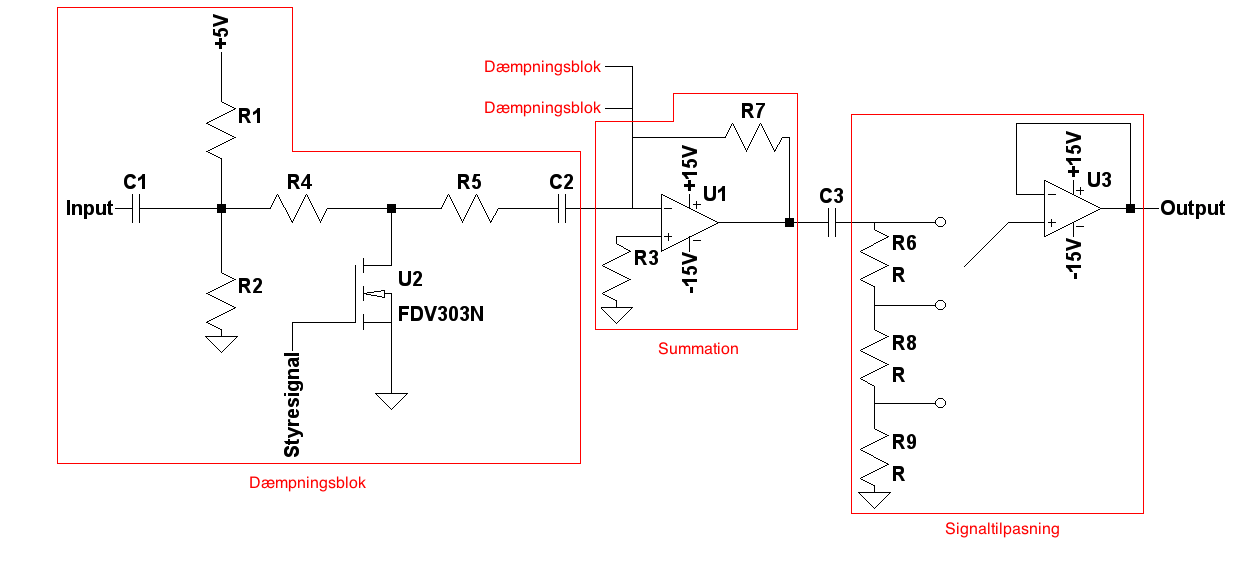
\includegraphics[width=\textwidth]{../rapport/teknisk/indgangsvaelger/signal-taend-sluk.png}
\label{fig:indgangsvaelger-overordnet}
\end{figure}
\end{frame}

\begin{frame}{Indgangsvælger - Styring}

\begin{figure}[h]
\centering
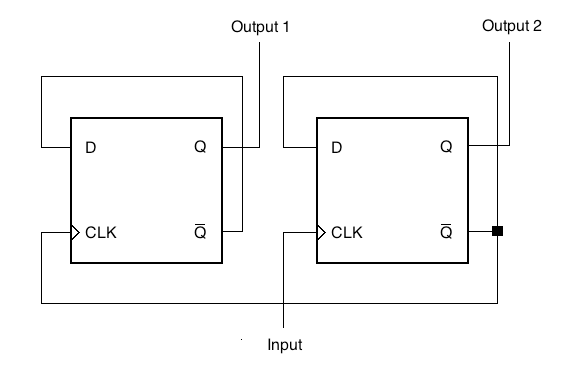
\includegraphics[scale=0.4]{../rapport/teknisk/indgangsvaelger/flipflop.png}
\label{fig:indgangsvaelger-flipflop}
\end{figure}
\end{frame}

\begin{frame}{Indgangsvælger - Simulering}
\begin{figure}[h]
\centering
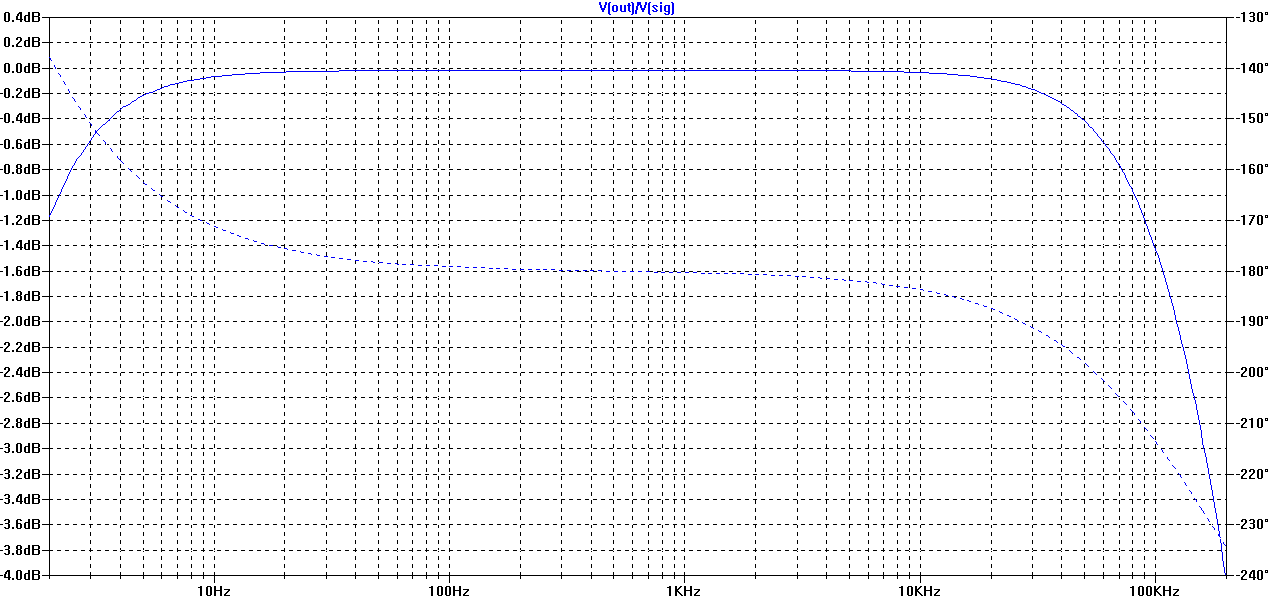
\includegraphics[width=\textwidth]{../rapport/teknisk/indgangsvaelger/simulering/frekvenskarakteristik.png}
\label{indgangsvaelger_frekvenskarakteristik}
\end{figure}
\end{frame}

\begin{frame}{Indgangsvælger - Måling}
\begin{figure}[h]
\centering
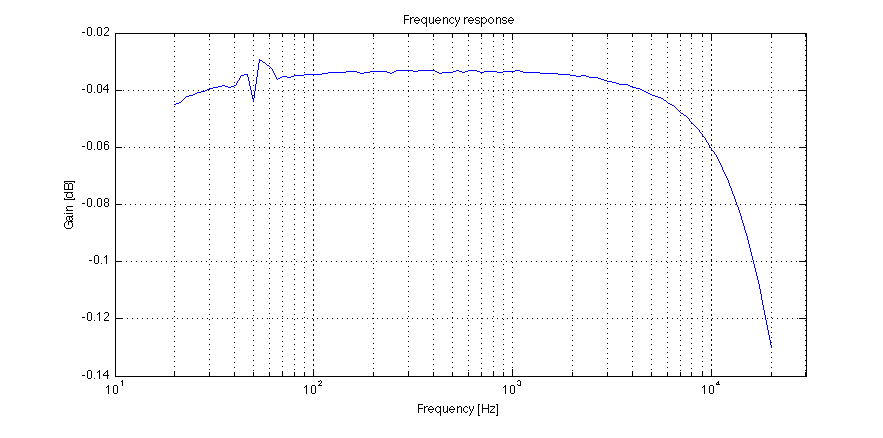
\includegraphics[width=\textwidth]{../rapport/maalerapporter/indgangsvaelger/Indgangsvlger-mic-200mv-frek.png}
\label{fig:indacc:frek200mv}
\end{figure}
\end{frame}

\begin{frame}{Indgangsvælger - Måling}
\begin{figure}[h]
\centering
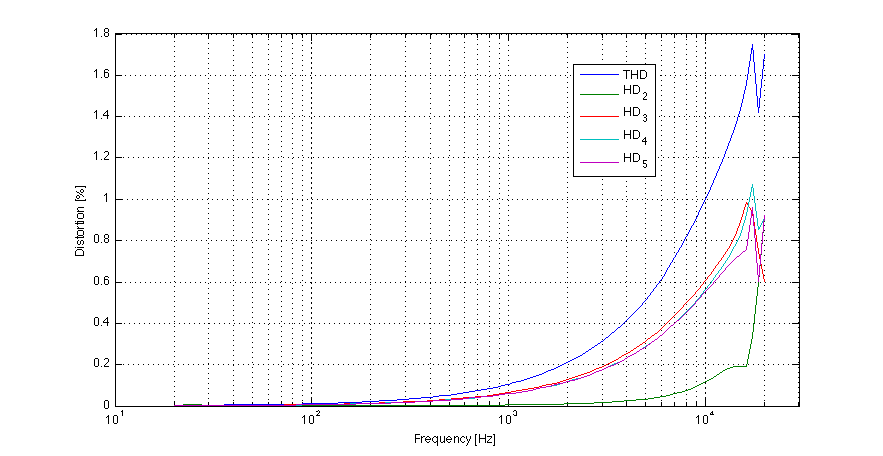
\includegraphics[width=\textwidth]{../rapport/maalerapporter/indgangsvaelger/Indgangsvlger-mic-2v-thd.png}
\label{fig:accind:thd2v}
\end{figure}
\end{frame}


\begin{frame}{Indgangsvælger - Oversigt}
\scriptsize{
\begin{table}[h]
\centering
\begin{tabular}{l|r|r}
\hline\hline
Område & Krav & Status \\
\hline\hline
Antal trin i & 4 & \checkmark \\
indgangsvælgeren & \\[4pt]
Indgangsimpedans & \> 22 k\ohm & \checkmark \\[4pt]
Frekvensgang & \< 0,375 dB ved 20 Hz - 20 kHz, ref. 1 kHz & \checkmark \\
& \< 0,75 dB fra 20 Hz til 63 Hz & \checkmark\\
& \< 0,75 dB fra 12,5 kHz til 20 kHz & \checkmark\\[4pt]
Dæmpning af slukket & \> 50 dB ved 1 kHz & \checkmark \\
indgangssignal & \\
\hline\hline
\end{tabular}
\label{tab:krav_indgangsvaelger}
\end{table}
}
\end{frame}

\section{Volumenkontrol}
\label{valg_volumenkontrol}
Kravet til styringen af volumenkontrol er sat til at dette skal foregå digitalt. Begrundelsen herfor ligger i projektets undertema, $"$High Fidelity (Hi-Fi) forstærker med digital styring$"$, og begrundes derfor ikke yderligere. Til bestemmelse af den maksimale dæmpning volumenkontrollen skal være i stand til, bruges samme krav som for slukkede signaler, altså 50 dB, som bestemt i afsnit \ref{standarder}. Volumenkontrollen skal derfor kunne dæmpe fra  0 dB til 50 dB. Desuden vælges størrelsen af hvert niveau til 1 dB, da dette er den mindste forskel et menneske kan opfatte i lydniveau \cite{lidt_om_lyd}. Dette sætter ydermere krav til at displayet, som opbygges af 7-segmenter, skal bestå af to 7-segmenter.\\
Volumen skal kunne justeres via trykknapper på HiFi-forstærkerens frontpanel, hvor det også skal være muligt at aflæse det øjeblikkelige volumenniveau.  


%Implementering
%\chapter{Implementering}
\label{implementering}


%Accepttest
\chapter{Samlet accepttest}
\label{acceptest}
Efter systemet implementeredes, blev der udført målinger, som vist i appendiks \ref{maaling_hifi}. Ud fra disse kan der konkluderes at systemet lever op til størstedelen af de opstillede krav. 

\begin{table}[h]
\centering
\begin{tabular}{l|r|l|r}
\hline\hline
Område & Krav & Betingelse(r) & Status \\
\hline\hline
\multicolumn{4}{c}{\textbf{Teknisk:}} \\\hline
Forstærkerklasse & AB & & \checkmark\\[4pt]
Total Harmonic & < 1 \% & & $\mathcal{X}$ \\
Distortion & & $\circ$ < 0,5 \% i forforstærker & \checkmark\\
& & $\circ$ < 0,5 \% i effektforstærker & $\mathcal{X}$\\
& & $\circ$ Begge i effektområde & \\
& & ~~~fra 0 til -26 dB & \\[4pt]
Frekvensgang & 20 Hz - 20 kHz & $\circ$ $\pm$ 1,5 dB ved ref. 1 kHz & \checkmark\\
& & $\circ$ < 3 dB dæmpning & \\
& & ~~~fra 20 Hz til 63 Hz og  & \\
& & ~~~fra 12,5 kHz til 20 kHz & \\[4pt]
Indgangstyper & Linie og mikrofon & $\circ$ Med $"$Monacor & \checkmark \\
& & ~~~MCE-4000$"$ mikrofon & \\[4pt]
Antal trin i & 4 & & \checkmark\\
indgangsvælger & & & \\[4pt]
Dæmpning af slukket & > 50 dB & $\circ$ Ved 20 Hz - 20 kHz & \\
indgangssignal & & & \\[4pt]
Indgangsimpedans i & > 22 k\ohm & & \checkmark \\
liniesignalsindgang & & &\\[4pt]
Indgangsimpedans i & > 5 k\ohm & & \checkmark \\
mikrofonsignalsindgang & & & \\[4pt]
Equalizer-bånd & 3 & & $\mathcal{X}$ \\[4pt]
Styring af volumen- & Digital & & $\mathcal{X}$\\
kontrol & & &\\[4pt]
Dæmpningsområde i & 0 dB - 50 dB & $\circ$ 1 dB per niveau & \checkmark \\
volumenkontrol & & & \\[4pt]
Udgangseffekt & > 20 W & $\circ$ I 8~\ohm-højtaler & $\mathcal{X}$ \\[4pt]
Udgangssignaltype & Mono & & \checkmark \\[4pt]
Kortslutningsstrøm & 3 A & $\circ$ Som peakstrøm & $\mathcal{X}$ \\
i udgangen & & & \\\hline
\multicolumn{4}{c}{\textbf{Frontpanel (input):}} \\\hline
Indgangsvælger & Èn trykknap & & \checkmark\\[4pt]
Volumenkontrol & To trykknapper & & \checkmark \\[4pt]
Equalizer & Èn drejeknap pr. bånd & & $\mathcal{X}$ \\\hline
\multicolumn{4}{c}{\textbf{Frontpanel (output):}} \\\hline
Indgangsvælger & To lysdioder & $\circ$ Én per indgang & \checkmark\\[4pt]
Volumedisplay & To 7-segmenter & & \checkmark \\[4pt]
Visualizer & 6 lysdioder & $\circ$ 2 grønne, 2 gule, 2 røde & $\mathcal{X}$ \\
\hline\hline
\end{tabular}
\caption{Status af krav for hele systemet}
\label{tab:kravspec:accept}
\end{table}

%Konklusion
\chapter{Konklusion}
\label{konklusion}

Formålet med dette projekt var at designe en HiFi-forstærker med digital styring. Målet var at designe en forstærker med to indgange, mikrofon og liniesignal, forforstærker, indgangsvælger, volumenkontrol, equalizer, visualizer og effektforstærker. Disse moduler skulle leve op til kravspecifikationen, som består af gængse standarder og krav bestemt af projektgruppen. 
Alle moduler undtagen tonekontrollen blev designet og simuleret. Equalizer og visualizer blev udeladt på grund af tidsmangel. Kortslutningssikringen er det eneste modul som ikke blev bygget og testet grundet at det indledende design var fejlbehæftet og tidsmangel. De resterende moduler er bygget og testet, samt blevet vurderet med udgangspunkt i de opsatte krav. 
Forforstærkeren og indgangsvælgeren bestod alle de opstillede krav. Volumenkontrollen var fejlbehæftet da tælleren ikke var konsistent i op og nedtælling samt at den har 52 trin, hvor kravet var 51. 
Effektforstærkeren overholdt alle kravene bortset fra at den dæmpede for meget indenfor frekvensområdet 20 Hz - 20 kHz. 

Efter at alle moduler var blevet testet hver for sig blev HiFi-forstærkeren implementeret og testet. Testene på det samlede system viste at ingen af de opsatte krav blev overholdt. 

\bibliographystyle{plain}
\bibliography{referencer/referencer}

\listoffixmes

\end{document}